\documentclass[a4paper,11pt]{article}
\usepackage{datetime}
\usepackage{csquotes}
\usepackage[style=numeric,sortcites=true,sorting=none,backend=biber]{biblatex}
\usepackage[parfill]{parskip}
\usepackage{fancyhdr}
\usepackage{graphicx}
\usepackage{subfig}
\usepackage{hyperref}
\usepackage{rotating}

\usepackage{amsthm}
\usepackage{soul}
\usepackage{commath}
\usepackage{mathtools}
\usepackage{array}

\addbibresource{../refs/SYB Exploratory Clustering.bib} % The file containing our references, in BibTeX format

\graphicspath{ {../structure/}{/home/ejuzovitski/Documents/master_thesis/structure/gantt/}}
\pagestyle{fancy}
\newcommand{\structure}{Project Specification and Schedule}
\newcommand{\mail}{emiljuz@kth.se}
\newcommand{\me}{Emil Juzovitski}
\newtheorem*{remark}{Remark}


\setlength{\headheight}{14pt}


\lhead{\structure}
\rhead{\mail}

\begin{document}
\section*{Project Specification}
\addcontentsline{toc}{section}{Project Specification}

\section{Formalities}

\subsection{Preliminary Thesis Title}

Using clustering analysis for song categorization and
music genre exploration on mixed data.

\subsection{Name and Email}

Emil Juzovitski - emiljuz@kth.se

\subsection{Supervisor @EECS}

Johan Gustavsson - johangu9@kth.se

\subsection{Name of the principal and name of the supervisor at the
principal's workplace}

\begin{itemize}
\item
  \textit{(Principal)} Soundtrack Your Brand
\item
  \textit{(Supervisor)} Omar Marzouk - Omar@soundtrackyourbrand.com
\end{itemize}

\subsection{Current Date}

\today

\pagebreak

\section{Background and Objective}

\subsection{Background}

This thesis is on the research topic of clustering analysis on mixed data. Clustering analysis is the term used for unsupervised learning
techniques that tries to group data of multiple dimensions together if
they are similar.\cite{doi:10.1002/9780470316801.ch1}. Mixed data refers to data being both categorical and numerical \cite{doi:10.1002/9780470316801.ch1,Jia2018,CHEUNG20132228,CHEN2016271}

The principal is a music streaming platform
company specializing in providing music for retail businesses. The
platform saves the customer time by automating their music selection. The
retail customer picks characteristics e.g. \textit{energy, genre, sound} that fit their brand. Sets of songs (playlists) are automatically generated for the customer to play based on the chosen characteristics.

With the tool of clustering a belief is that
similar songs can be grouped together, and, potentially uncover themes
in similar songs. If a cluster is determined to have a theme, songs of that
cluster can be assigned a categorical label, that is, the theme. Given
enough themes, the previously unlabeled dataset becomes labeled. A resulting effect is
that the now labeled data can be used for supervised learning. In addition to creating a supervised dataset, clustering songs can help playlist composers employed by the company to find candidate songs for tailored playlists reducing the time needed to find songs for a playlist.

For the purpose of this project, a dataset of songs will be used, it includes more than $5\cdot10^7$ data entries. The attributes of each song are metadata and an audio-embedding characterizing the song. Together they make up more than 100 attributes that are \textit{mixed}.

As stated above, the data is mixed, i.e. the attributes are of different
data types. While interval-scaled distances (numerical) can be measured well through
the Euclidean distance measurement, \textit{categorical data} cannot be measured in the same fashion without information loss.  There are suitable distance measurements for \textit{categorical data} but these measurements are inherently unsuitable for interval based data. \textit{Generalized Gower distance(daisy function)} \cite{doi:10.1002/9780470316801.ch1} is one way to generalize distance measurements on mixed data. Still, traditional clustering algorithms only implement one data type distance measure, as a mixed data distance often comes with an increase of complexity on the general algorithm. % A main objective of the thesis is to compare different
% clustering approaches and evaluate which approaches is most suitable for
% the given dataset both in terms of clustering quality(using the
% silhouette coefficient) and scalability(time to cluster different sample
% sizes of the dataset). Other topics include preprocessing and sampling
% from the clusters.

% An additional objective is to cluster and pre-process in such fashion that in terms o
% \textit{direct evaluation} from the top 100 clusters at least 10-25 have themes from the eyes of the music experts.


\subsection{State-of-The-Art}
%% State of the attributes
While there is a rich source of papers on clustering approaches for numerical data, the same cannot be said for mixed clustering algorithms. Below is a brief summary of some mixed data approaches:

Mixed data clustering algorithms are mostly adoptions of previously existing algorithms. The perhaps most well known algorithm is a modification on \textit{K-means} clustering called \textit{K-prototype} \cite{Huang97clusteringlarge} --- it introduces a similarity measurement for mixed data . The similarity measure can be found in equation \ref{eq:1}. $w_l$ determines how important categorical data is compared to its numerical counterpart for cluster $l$. A simplification is made in the algorithm replacing local $w_l$ for each cluster $l$ with a single global weight $w$. The weight $w$ is a user-defined input.
%while obtaining the same time complexity of \textit{O(nkdi)}%

\begin{equation}
\label{eq:1}
d(X_i, C_l) = \sum_{j=1}^{m_r}( x_{ij}^{u} - c_{lj}^{u} )^2 +
  w_l \sum_{j=1}^{m_c}\delta( x_{ij}^c, c_{lj}^c )
\end{equation}

% where:
% \begin{conditions}
%   C_l   & Prototype C_l \\
%   w_l     &  Weight of categorical attributes for C_l \\
%   m_r     &  Number of numerical attributes \\
%   m_c     &  Number of categorical attributes \\
%   x_{ij}^k  & Attribute j^k of X_{i} \\
% \end{conditions}



\textit{K-prototype} has the same problems that can be assigned to \textit{K-means}, additionally it has problems that the new similarity measure introduces, stemming mostly from the user specified weight input. State-of-the-art algorithms built on \textit{K-prototype} try to solve a few of the problems embedded in \textit{K-prototype} algorithm. Two fundamental problems are the requirement of k as a user input as well as the that the algorithm assumes all attributes to be of equal importance \cite{CHEUNG20132228}\cite{huang2005automated}.

% A fundamental problem with k-means is High-dimensional data. It is often the case that a subspace of that data is important

In \cite{CHEUNG20132228} the \textit{OCIL} algorithm is introduced. The problem of requiring a $k$ --- the number of clusters --- as an input is solved through the use of competitive learning. A new unified and more precise similarity measure is also introduced. The argument for the similarity measure is that all numerical values are seen as one single vector requiring one weight, while categorical values require one weight each. (I'll add the similarity measure later in the process, see page 4 in the cited paper)

The authors of \cite{CHEUNG20132228} iterate on their solution in \cite{Jia2018} taking a soft subspace approach --- assigning weights to all attributes differently depending on the cluster and measuring each attributes' contribution to a cluster \cite{DENG201684}  --- to allow unique cluster weights without the need of weights defined by the user while still allowing a reasonable performance. (I'll expand on this much more later in the process)


A density based-approach is taken in \cite{CHEN2016271} for clustering mixed data. Cluster centers are found by taking field intensity distance to account. With the now known centers, data is clustered. The algorithm is then extended for streaming data.

An ensemble method is introduced in \cite{DBLP:journals/corr/abs-cs-0509011} where any two clustering methods for numerical and categorical data respectively are used to to cluster the data-types separately. The clustering results are then merged on the basis that clustering results --- even from numerical --- are always categorical.

As the information on mixed-data is sparse it is not clear cut what clustering methods to use. A person not in the know-how could easily result in converting categorical data to numerical revoking information loss that could easily been avoided using a mixed-data technique \cite{doi:10.1002/9780470316801.ch1}. Mixed-data techniques are not as fast as state-of-the-art numerical-clustering algorithms but make up by being compatible with mixed data. Above algorithms have capabilities to handle real-world situations where inputs are not known, and, different clusters have different attribute dependence. \textcite{Jia2018} in particular solves most if not all problems that occur when a new mixed dataset has to be clustered, while still being relatively fast.

\subsection{Evaluation}
In data-mining evaluation often cares about determining whether items are relevant or not \cite{manning2010introduction}. In the case of clustering we want to evaluate whether resulting clusters are relevant or not.

There are two main ways of which clustering are evaluated: internal- and external-criterion \cite{manning2010introduction}
. In some research the categories are extended with the relative-criterion.\cite{Halkidi2002}

The Internal criterion is an unsupervised validation approach and can be described as evaluating the results without respect to external information \cite{Halkidi2002}. The average \textit{silhouette coefficient} upon all datapoints $\overline{s}_{co}$ shown in \ref{eq:avg_s}, is one way to evaluate the internal criteria \cite{ROUSSEEUW198753}. A single silhouette coefficient is shown in \ref{eq:sil}, it looks at a data points intra-cluster similarity --- similarity to points within the same cluster, and, inter-cluster similarity --- similarity with pointstside of the cluster. $\overline{s}_{co}$ goes between -1 and 1 where a high value (close to 1) indicates a natural clustered dataset.

When $s_{co}(X_i)$ is a high value (close to 1) a point is well clustered i.e. the intra-cluster similarity is high relative to the inter-cluster similarity \cite{ROUSSEEUW198753}. The same reasoning is extended to $\overline{s}_{co}(\mathcal{D})$ where a high value is a well clustered dataset.

\begin{align}
  d_{avg}(X_i,C_l) &= \frac{\sum_{X_k \in C_l}d(X_i,X_k)}{Count(X_k \in C_l)} \\
  a(X_i) &= d_{avg}(X_i,C_a) \textit{ , where } (X_i \in C_a) \\
  b(X_i) &= min_{C \neq C_a}(d_{avg}(X_i,C)) \\
 \label{eq:sil}
  s_{co}(X_i) &= \frac{b(X_i) - a(X_i)}{max(a(X_i), b(X_i)} \\
\label{eq:avg_s}
  \overline{s}_{co}(\mathcal{D}) &= \frac{\sum^{N}_{i=1} s_{co}(X_i)}{N}
\end{align}

External criterion is supervised validation approach and can be described by the following sentence: Validation of the results by imposing a pre-defined structure on the dataset i.e. data not used for generating the clustering results \cite{Halkidi2002}. As clustering analysis is an unsupervised learning method, it is often hard to assess the criteria --- There is often no test data available for a new dataset. Still, to quantify how well the clustering approach works on a new dataset defining a ground truth is essential. One way is to use judges, experts in the field \cite{manning2010introduction}. Given a ground truth an external measurement can be deployed.

Purity is a measurement for the external criterion. It measures the ratio of the most dominant class in a cluster. The data-points are labeled with a class beforehand on the ground truth \cite{manning2010introduction}. Equation \ref{eq:purity} defines the measurement. The equation does not penalize small clusters as such small clusters produces a high score.

\begin{equation}
  \label{eq:purity}
  P(W, C) = \frac{1}{N}\sum_{k}max_{j}\abs{w_k \cap c_j}
\end{equation}
Where:\newline
$W = \{w_1,w_2,...,w_k\}$ is the set of clusters, and,
$C = \{c_1,c_2,...,c_k\}$ is the set of clusters.

Another measurement is the \textit{$F$-measure} shown in \ref{eq:f-measure}. Where P is the precision defined in \ref{eq:precision} and R, recall is defined in \ref{eq:recall}. The measurement is a way to take account both Precision and Recall. The balanced \textit{$F$-measure} is called the \textit{$F_1$-measure} and is defined in \ref{eq:f1-measure}. It weighs the impact of precision and recall the same.
\begin{align}
  \label{eq:precision}
  P &= \frac{TP}{TP+FP} \\
  \label{eq:recall}
  R &= \frac{TP}{TP+FN} \\
  \label{eq:f-measure}
  F_\beta &= \frac{(\beta^2 + 1) \cdot P \cdot R)}{\beta^2 \cdot P + R} \\
  \label{eq:f1-measure}
  F_{\beta = 1} &= \frac{2 \cdot P \cdot R}{P + R}
\end{align}
Where:\newline
$TP$ are true positives, $FP$ false positives, $FN$ false negatives, and, $\beta$ is a weight between $P$ and $R$, a $\beta > 1$ emphasizes the $R$.

\subsection{Interest and Objective}

There are two main interests of the company:

\begin{itemize}
\item
  The company wants to find a way to efficiently create supervised
  training data. Clustering datapoints/songs would allow to categorize
  data and append an approximate label to each data point. Supervised
  training data would unlock the usage of supervised learning for
  further projects.
\item
  Playlists are handpicked by music composers which requires extensive labour. Clustering can help to
  reduce the \textit{Searching} done by the composers by giving them
  \textit{candidate songs} for a cluster/themes, resulting in less time
  focused on irrelevant songs.
\end{itemize}

From a thesis standpoint the objective is to measure the performance improvements by using a state-of-the-art mixed clustering method in comparison with a unit conversion approach on the given dataset. In addition, an objective is that the chosen mixed-clustering algorithm can produce clusters of which playlist composers agree to have a theme.

\subsection{Research Objective}

\section{Research Question and Method}

% \textbf{Original} \textit{\st{How can state-of-the-art clustering be used to categorize music, given a mixed attribute dataset of songs whose attributes are metadata and an audio embedding?}}

% \textbf{Alt 1. Longer} \textit{What clustering performance increase does the usage of state-of-the-art mixed clustering create in comparison to using a method in which categorical data is converted to numerical data and later clustered with a numerical clustering method on the given mixed dataset of songs with metadata and an audio-embedding?}

\textit{What clustering performance increase does the usage of state-of-the-art mixed clustering create in comparison to a method in which categorical data is converted to numerical data on the given mixed dataset of songs with metadata and an audio-embedding?}

% \textit{To which extent does state-of-the-art mixed data clusteringstperform --- clustering performance evaluated by a judge --- a method in which categorical data is converted into numerical data and later clustered on a real-world mixed dataset containing songs with metadata and an audio-embedding?}
(There is no need to choose two different algorithms, mixed data algorithms (i.e. OCIL) behave like a numerical algorithm on numerical data.)

% \subsection{Specified problem definition}

% The challenge arises from the dataset being real-world, where datasets
% are often of mixed data types as it is for this dataset. Steps differing from clustering numerical are
% necessary to cluster mixed data as the majority of clustering
% algorithms are implemented using the \textit{Euclidean distance measurement.}It is therefore necessary to look at existing mixed data algorithms that solve the problem of the dataset. What does not differ from numerical clustering approaches is the problems of validating the results on a new dataset without knowing the optimal clusters a priori.

% % Move this to evaluation


\subsection{Examination Method}

\subsubsection{Dataset}

A dataset of \textit{songs} will be used. It includes more than 50 million
entries with each song entry holding hundreds of attributes. Attributes
of a song is its metadata as well as its audio embedding: anstput from
a machine learning algorithm characterizing the audio of the song. Not
all attributes are \textit{interval-scaled (continuous-linear, numerical)}. The metadata
attributes are e.g. \textit{release year (ordinal), BPM (ordinal),
explicit (binary), artist, gender (binary)}. The embedding is a vector of
audio properties of the song with dimensionality in the hundreds. What
each attribute means is unknown, the value of the attribute is
interval-scaled.

Two caveats are that certain songs can be missing one or more attributes, and, certain songs can have multiple values for one attribute e.g. \textit{genre}.


\subsection{Computation and Language}

Google Cloud will be the computation source. To allow possible
distributed implementations, code will be written in Python and, Apache
Beam or Apache Spark.

% \subsubsection{Method (old)}

% \begin{itemize}
% \item
%   Preprocessing of data
%   \begin{itemize}
%   \item
%     We cannot assume all features allow clusteringst of the box.
%     Certain features need to be divided, some hashed, some just do not
%     work(images) and so forth, some are irrelevant and need to be thrown
%    st.
%   \item
%     Some features are inadvertently more important than others,
%     weighting is a simple solution however, it is not clear how to find
%     what features are important without resulting to complex solutions
%     such as using a dimension reducing neural network.
%   \end{itemize}
% \item
%   Choosing Clustering algorithms
%   \begin{itemize}
%   \item
%     Different types of clustering algorithms will be compared
%     \textit{CLARANS, DBSCAN, QuickShift, ROCK} Algorithm etc.
%     \begin{itemize}
%     \item
%       Determining what is ideal for the dataset.
%     \item
%       Handling mixed data-types.
%       \begin{itemize}
%       \item
%         Finding specific mixed attribute algorithms e.g. K-prototypes that define a mixed data approach.
%       \item
%         Ensemble methods? e.g. \textit{DBSCAN} with \textit{ROCK}
%       \item
%         Ignoring the issue, conversion to Euclidean distance.
%       \item
%         Cluster on non-categorical, filter on the categorical as a
%         post-processing step.
%       \end{itemize}
%     \end{itemize}
%   \end{itemize}
% \item
%   Determining parameters for clustering
%   \begin{itemize}
%   \item
%     Partitioning algorithms e.g \textit{K-means, CLARANS} assume \textit{k}
%     (the amount of clusters) is known beforehand. This is not the case
%     for this thesis and so \textit{k} approximation is necessary (that
%     is not too computationally heavy).
%     \begin{itemize}
%     \item
%       Sampling is an option.
%     \item
%       Another solution is to use another clustering approach such as
%       density based clustering e.g. \textit{DBSCAN} that does not require
%       \textit{k}.
%     \end{itemize}
%   \end{itemize}
% \item
%   Implementing Clustering algorithms
% \item
%   Evaluating clustering approaches
%   \begin{itemize}
%   \item
%     Comparing the inner criterion.
%   \item
%     Creating a \textit{purity} test
%     \begin{itemize}
%     \item
%       Ranking clusters by silhouette coefficient
%     \item
%       Sampling from top resulting clusters
%     \end{itemize}
%   \end{itemize}
% \end{itemize}


\subsection{Expected scientific results}

Clustering accuracy is relative. While we can measure the inner
criterion through e.g. silhouette coefficient, a high silhouette does not
necessarily translate into clusters with themes that make sense from an
end-user standpoint. Instead a external evaluation --- the supervised evaluation, can be used by asking the
end-user about the resulting clusters and using the measurement of
\textit{purity.}

My hypothesis is that both the inner criterion and external criterion will see an improvement by using a mixed-data clustering algorithm. I think a purity increase over $10\%$ will be achieved.

\section{Evaluation and News Value}

\subsection{Evaluation}
For the internal criterion the \textit{average silhouette coefficient} will be used. For the external criterion the \textit{purity} measure will be used.

In order to use any external criteria, a ground truth estimate is necessary. There are various options in this thesis on how to generate it. There are music composers available, there are $10^3$ of tailored playlists, and, there is also a genre attribute that can be used as the ground truth if it is excluded from the clustering generation.

If the genre is excluded, data can get labeled on the genre. A basic purity test can then be done: finding the amount of songs with the dominant genre label in each cluster and dividing that with the amount of points in those clusters.

If we depend on the composers and want to create a purity measurement, we would have to let the composers decide if there is a theme in a cluster as well as deciding which songs are apart of that theme. To lessen the workload we could sample some clusters, and some songs of those clusters.

If we use the playlist to create a purity measurement, we would have to let the composers decide if there is a theme in a cluster as well as deciding which songs are apart of that theme. To lessen the workload we could sample some clusters, and some songs of those clusters.

The genre exclusion validation do not require any additional work, and, is less subjective. It also generates more testing data than what composers could provide. The downside of the genre exclusion option is that genres could improve the clustering results if it would be used in the clustering process. On the other hand the exclusion forces \textit{new} themes/genres to be found.

The decision is to use genre exclusion with \textit{purity} for now as it is the most robust way the project can assert the external validity. An option for the project could be to use the composers on a sample of the dataset if it was decided later that it is too favorable not to cluster on the genre.

The objective is fulfilled if we obtain the internal and external validity measurements on a clustering result and can assess a performance difference on the dataset compared to a unit conversion approach.

%The external validity measure should
% The objective is fulfilled if we get a high internal on a majority of the clusters and a high external score on a subset of our most dominant clusters.

\subsection{News Value}

It is often the case in real world situations that the clustering
analysis is required to be done on data fetched from a database. A
database often stores data of different types and so the dataset to
cluster is often of mixed data types. This thesis takes a deep-dive into state-of-the-art mixed data clustering methods and proposes a clustering solution for categorizing songs on a dataset of mixed attributes. With mixed data clustering methods not being a familiar topic for many this thesis reintroduces the clustering category with a new real world dataset to show the current performance capabilities of the field.

\section{Pre-study}

% \textbf{Original. } Focus will be on clustering algorithms and everything around it, to be more specific: Unsupervised \textit{Single-machine}(for now) clustering methods.

% \textbf{New. } 
Focus will be on mixed data clustering algorithms that reduce the amount of user inputs, while still allowing a relatively high time-performance. Topics include: Subspace clustering and automatic K-variable detection.

\subsection{Finding information}

\subsubsection{Initial Keywords}

\textit{Clustering, Mixed data, Review, Pre-processing, soft subspace clustering, k-initialization}

\subsubsection{Method}

\begin{itemize}
\item
  Initially start with finding Review articles on state of the art
  clustering methods.
\item
  Go more in depth into algorithms suitable for dataset, look at
  original paper.
\item
  Find sources on pre-processing.
\item
  Search for mixed data solutions.
\end{itemize}

\subsection{Obtaining the necessary knowledge and preliminarily
references}

There are numerous steps in order to go from data tostput:


\begin{itemize}
\item
  The first step is data type assertion and conversion. What kind of
  data is the dataset? How do we measure it can we convert it.

  \begin{itemize}
    \item
      This topic is assessed by looking at how clustering is affected by
      data types and distance measurement.
    \item
      Current reference is \textit{Finding Groups In Data}(Kaufman, 1990)\cite{doi:10.1002/9780470316801.ch1}.
  \end{itemize}
\item
  The second step is to find suitable clustering algorithms. A way to
  start is to look at a review summarizing some of the highly used
  algorithms numeric of today. From there mixed data clustering algorithms will be searched for.
  \begin{itemize}
  \item
    Current reference for summary is \textit{Big Data Clustering: A
    Review} (Shirkhorshidi, 2014)\cite{Shirkhorshidi2014}.
  \item
    Current Numerical clustering algorithm references.
      \begin{itemize}
        \item \textit{CLARANS: A Method for Clustering Objects for Spatial Data Mining} (R.Ng, 2002)\cite{Ng2002},
        \item \textit{A Density-Based Algorithm for Discovering Clusters in
    Large Spatial Databases with Noise} (Ester, 1996)\cite{Ester1996}.
      \end{itemize}
  \end{itemize}
  \item
    Current Mixed attribute clustering algorithm reference.
      \begin{itemize}
        \item \textit{Clustering large data sets with mixed numeric and categorical values} (K-prototypes) (Huang, 1997)\cite{Huang97clusteringlarge},
      \end{itemize}
\end{itemize}

\section{Conditions and Schedule}

\subsection{List of resources}

\begin{itemize}
\item
  \textit{"Playlist Composers"} - Professional playlist makers.

  \begin{itemize}

  \item
    These professionals are full-time employees at the principal. It
    cannot be expected that they go through all songs and all clusters.
    However, going through samples of 10-100 top clusters is to be
    expected by the Music experts.
  \end{itemize}
\item
  Google Cloud
  \begin{itemize}
    \item Cloud computing
  \end{itemize}
\item
  Machine with over 100GB of memory

  \begin{itemize}
  \item
    With Google cloud any machine can be ordered up until terabytes of
    memory. Clusters of machines could also be ordered.
  \item
    For the principal it is expected that the thesis will need a
    machine/machines that matches the requirements from my side.
  \end{itemize}
\item
  Python Clustering Library

  \begin{itemize}
  \item
    Maybe pyclustering (https://github.com/annoviko/pyclustering)
  \item
    Maybe Spark MLLib
  \end{itemize}
\item
  Apache Beam/Apache Spark

  \begin{itemize}
  \item
    A distributed framework
  \end{itemize}
\end{itemize}

\subsection{Defined Limitations}

I will describe the attributes of the dataset that are of interest for
the thesis and its data types with the exception being the audio
embedding. How the audio embedding is created will not be mentioned
either due to company policy.

If a high performing mixed clustering method is not available, it could get excluded as an option for this thesis due to a limitation of time.

I could expand my limitations with time but for now, Constraint
Clustering, Neural Networks such as SOM will not be considered at the
time of writing.

\subsection{Collaboration with the principal}

The principal will:

\begin{itemize}
\item
  provide the dataset.
\item
  Provide extensive support and knowledge
  \begin{itemize}
    \item
      Guide me with decisions and ML problems.
    \item
      Discussions on results
    \item
      Might read my report but not main objective.
    \item
      Support on how to use the company resource eco-system
  \end{itemize}
\end{itemize}

\subsection{Schedule}
See \ref{fig:sch} in Attachments.

\newpage
\printbibliography[heading=bibintoc]
\newpage

\section*{Attachments}

\newpage
\thispagestyle{plain}
\begin{sidewaysfigure}[h!]
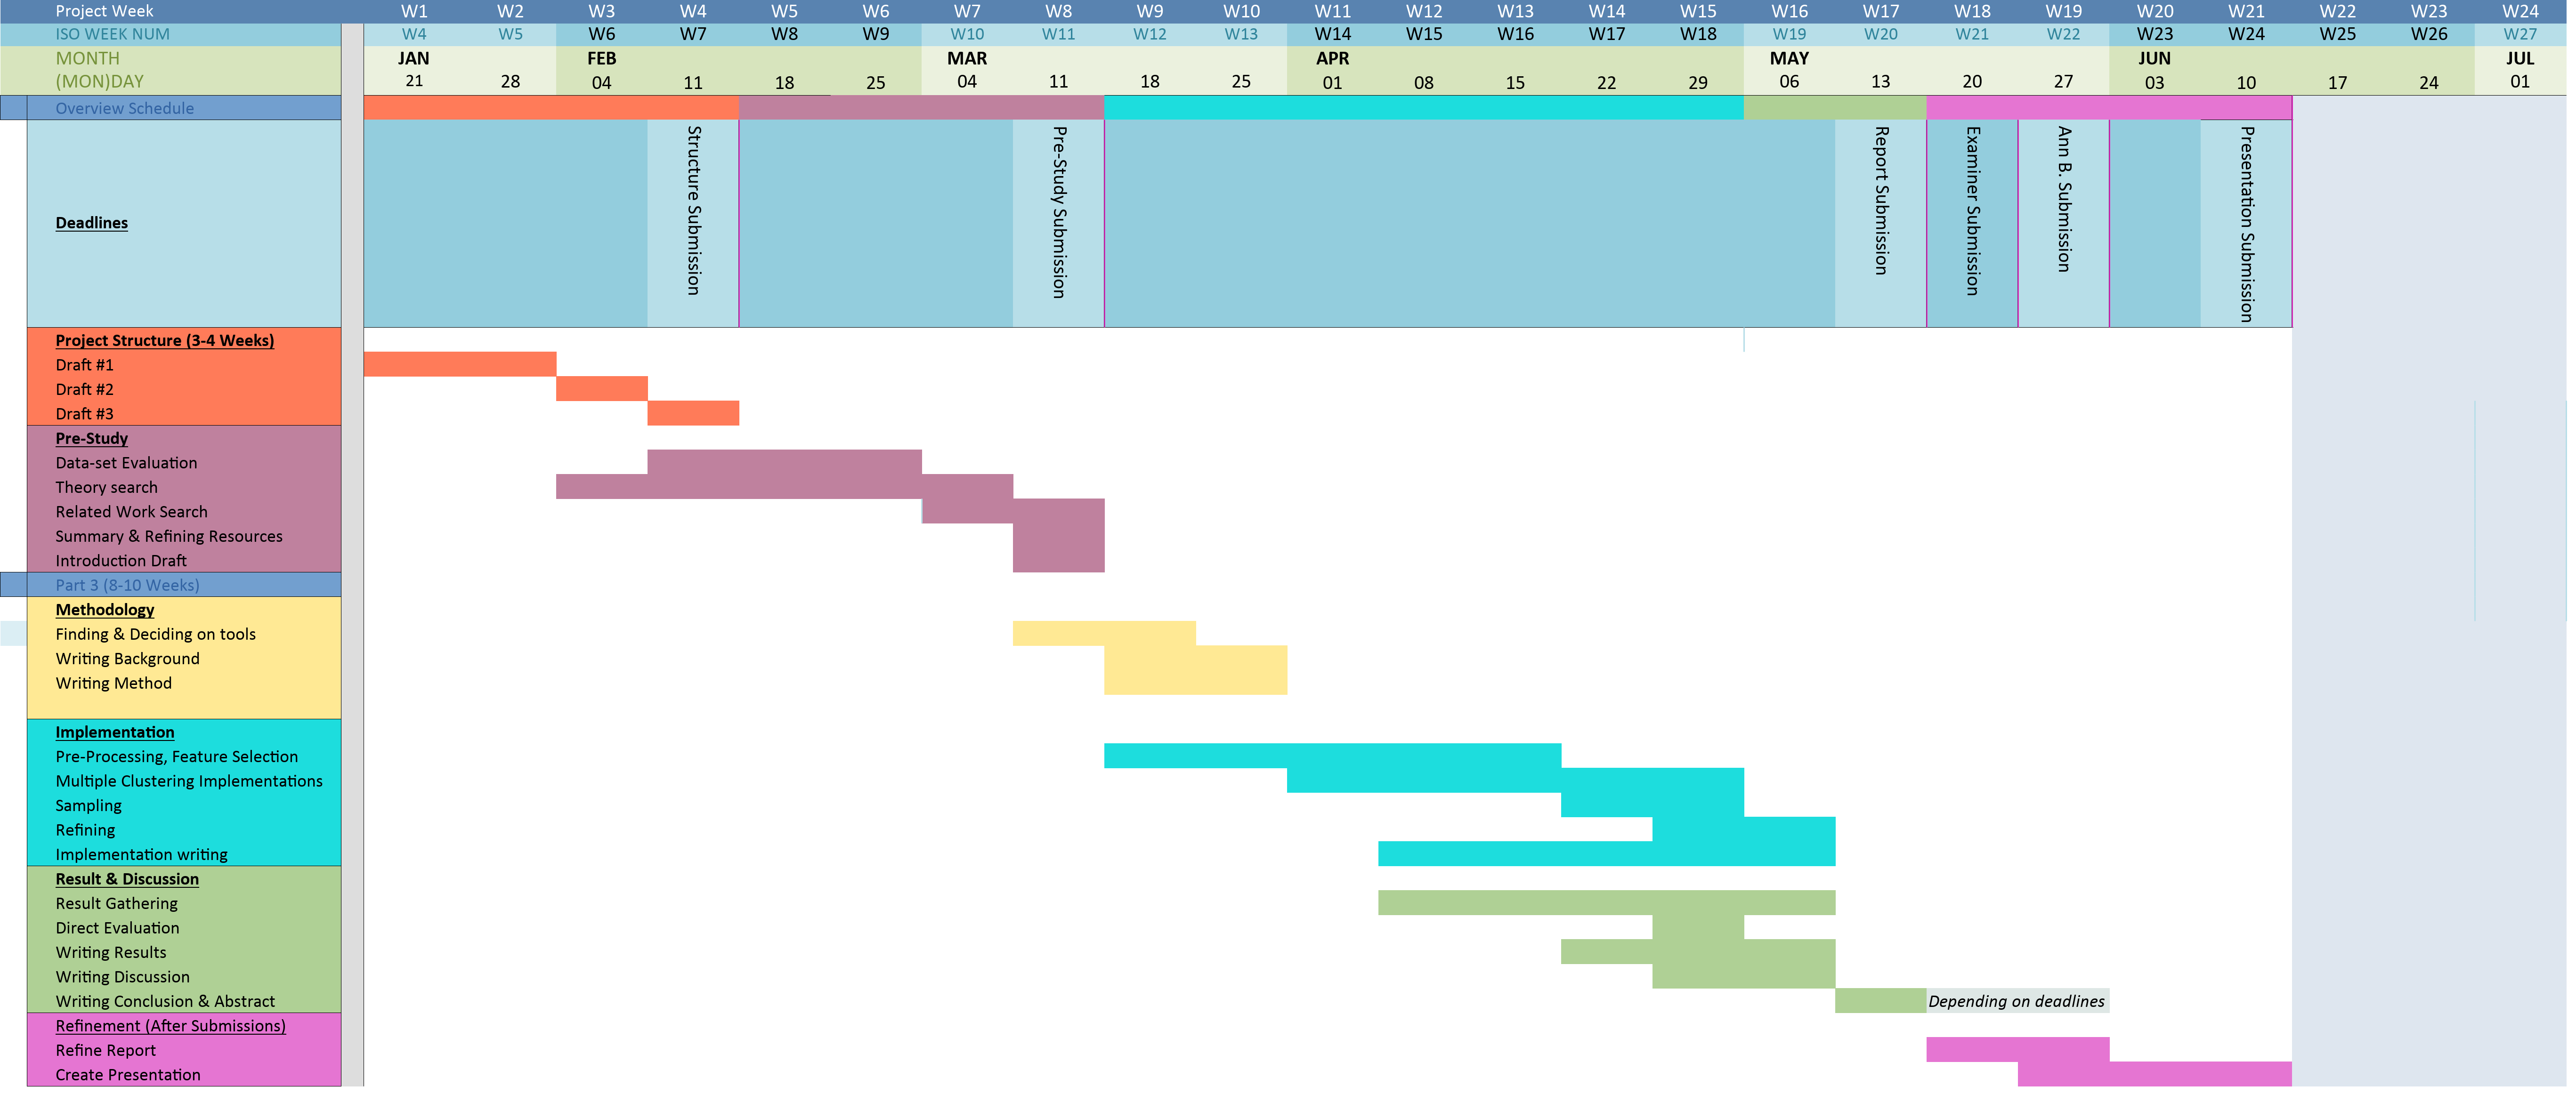
\includegraphics[height=0.45\textheight]{Grantt}
\caption{Preliminary Schedule}
\label{fig:sch}
\end{sidewaysfigure}
\newpage

\end{document}

